\documentclass[border=20pt]{standalone}
\usepackage{tikz}
\usepackage{amsmath}
\usetikzlibrary{calc,arrows.meta,angles,quotes}
\begin{document}
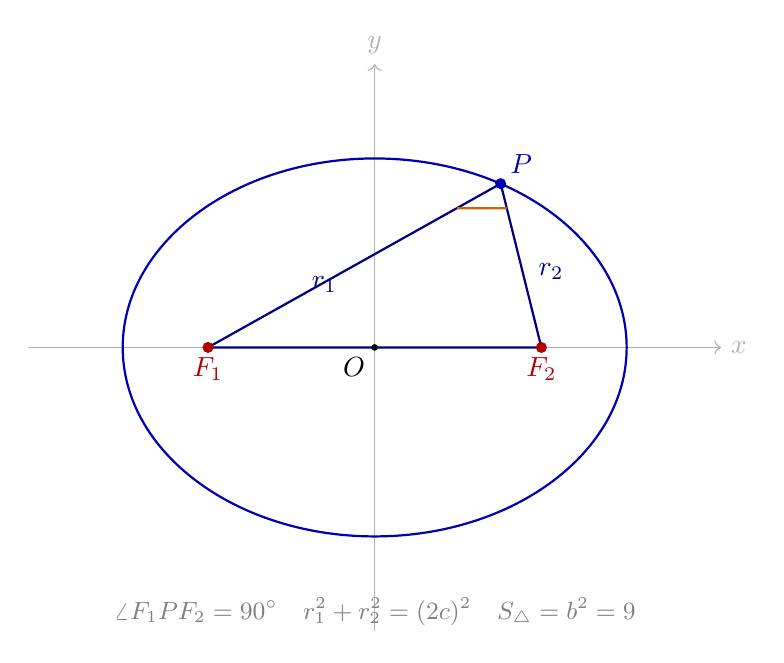
\begin{tikzpicture}[scale=0.8]
  % Axes
  \draw[->, gray!60, thin] (-5.5,0) -- (5.5,0) node[right] {$x$};
  \draw[->, gray!60, thin] (0,-4.5) -- (0,4.5) node[above] {$y$};

  % Ellipse: a=?, b=? (generic, use a=4, b=3 for visual)
  \draw[thick, blue!70!black] (0,0) ellipse (4 and 3);

  % Foci (±c,0)
  \coordinate (F1) at (-2.646, 0);
  \coordinate (F2) at (2.646, 0);
  \coordinate (O)  at (0,0);

  % Point P where ∠F1PF2 = 90° (on circle x^2+y^2=c^2 intersect ellipse)
  % For a=4,b=3: c=√7≈2.646, P ≈ (±2.2, ±2.5) — visually approximate
  \coordinate (P) at (2.0, 2.6);

  % Triangle
  \draw[thick, blue!50!black] (F1) -- (P) -- (F2) -- cycle;

  % Right angle marker at P
  \draw[orange!80!black, thick] ($(P)!0.15!(F1)$) -- ($($(P)!0.15!(F1)$)!0.15!($(P)!0.15!(F2)$)$) -- ($(P)!0.15!(F2)$);

  % Points
  \fill[red!70!black]  (F1) circle (2.5pt) node[below] {$F_1$};
  \fill[red!70!black]  (F2) circle (2.5pt) node[below] {$F_2$};
  \fill[blue!70!black] (P)  circle (2.5pt) node[above right] {$P$};
  \fill[black]         (O)  circle (1.5pt) node[below left]  {$O$};

  % Labels
  \node[blue!50!black] at (-0.8, 1.0) {$r_1$};
  \node[blue!50!black] at (2.8, 1.2)  {$r_2$};

  \node[text=gray, font=\small, align=center] at (0, -4.2)
    {$\angle F_1PF_2=90^\circ\quad r_1^2+r_2^2=(2c)^2\quad S_{\triangle}=b^2=9$};
\end{tikzpicture}
\end{document}
